The development of this program started by getting a proof of concept up and running without much regard for whether the system was well constructed. This was done to not get stuck in the planning phase and to get some code working as soon as possible. The idea was to try and identify a good workflow and how the musical structures could be implemented.


I wanted to test out how I could generate notes and visualize them as well as listen to audio of the notes generated. For this I used \textit{python} to generate \textit{lilypond}\footnote{lilypond is a text based musical typesetting language\cite{LilyPondMusicNotation}} files. From these files I was able to generate PDFs of sheet music as well as \textit{wave-files} to listen to how it sounds without having to play or sing it myself.

After the first iteration, lots of issues were observed and were put into the specifications for the second iteration which improved upon the model in various ways. Some important missing features were restricting the range so that an actual instrument can play it and the melody followed no structure.

\section{Software architecture}
  This initial software architecture can barely be called architecture. The first iteration works more like a script that generates a simple rhythm with the melody moving randomly in small intervals, 2nds and 3rds, analogous to a random walk only in one dimension.
  The system has musical representation of keys and spelling notes correctly regarding the key, but no phrasing or harmonic restrictions are implemented.

  Figure~\ref{fig:iter1_architecture} shows the structure of the first iteration. The pipeline is small and direct: the configuration is hard-coded in the main script, rhythm and pitch are generated independently for each voice, and the result is exported directly to LilyPond without a richer planning or constraint layer.

  \begin{figure}[htbp]
    \centering
    \resizebox{\textwidth}{!}{%
    \begin{tikzpicture}[
      >=Latex,
      font=\small,
      node distance=8mm and 10mm,
      stage/.style={
        draw,
        rounded corners=3pt,
        align=center,
        minimum width=0.42\textwidth,
        minimum height=10mm,
        fill=gray!8
      },
      support/.style={
        draw,
        rounded corners=3pt,
        align=center,
        minimum width=0.24\textwidth,
        minimum height=9mm,
        fill=blue!6
      },
      output/.style={
        draw,
        rounded corners=3pt,
        align=center,
        minimum width=0.24\textwidth,
        minimum height=9mm,
        fill=green!8
      },
      arrow/.style={
        -{Latex[length=2.3mm]},
        thick
      }
    ]

      \node[stage] (input) {User input and hard-coded configuration\\key, mode, bars, time signature, voice list};
      \node[stage, below=of input] (main) {\texttt{main.py}\\loops through voices and coordinates generation};
      \node[stage, below=of main] (generator) {\texttt{generators/generator.py}\\random rhythm filling and random scale motion\\by 2nds and 3rds};
      \node[stage, below=of generator] (melodies) {\texttt{Melody} objects per voice\\notes and rhythm attached after generation};
      \node[stage, below=of melodies] (render) {\texttt{out/lilypond.py}\\ChoirStaff assembly, LilyPond export,\\PDF/MIDI generation and audio playback};

      \node[support, left=18mm of generator] (music) {\texttt{core/music.py}\\\texttt{Key}, \texttt{Note}, \texttt{Melody}\\and scale helpers};
      \node[support, right=18mm of generator] (voices) {voice configuration\\clef and allowed rhythm values\\for each generated line};

      \node[output, below left=10mm and 10mm of render] (ly) {\texttt{.ly} source};
      \node[output, below=10mm of render] (pdf) {cropped \texttt{.pdf}};
      \node[output, below right=10mm and 10mm of render] (audio) {\texttt{.midi} and \texttt{.wav}};

      \draw[arrow] (input) -- (main);
      \draw[arrow] (main) -- (generator);
      \draw[arrow] (generator) -- (melodies);
      \draw[arrow] (melodies) -- (render);

      \draw[arrow] (music.east) -- (generator.west);
      \draw[arrow] (voices.west) -- (generator.east);

      \draw[arrow] (render) -- (ly);
      \draw[arrow] (render) -- (pdf);
      \draw[arrow] (render) -- (audio);

    \end{tikzpicture}%
    }
    \caption{Architecture of the first iteration melody generator. The first proof of concept uses a small script-driven pipeline where rhythm and pitch are generated per voice and then exported directly through LilyPond.}\label{fig:iter1_architecture}
  \end{figure}

\section{Implementation}
  This first iteration was a very primitive handling of generating music. It had very few constraints on the melody and contained little to no metadata on the music which made it unsuitable for actual music.

  In practice the code worked by taking a few fixed settings in the main script, generating one voice at a time, and then exporting the result directly to LilyPond. Rhythm and pitch were generated separately, and each voice was unaware of the others. This was enough to get visible and audible output quickly, but it also meant that almost none of the larger musical structure was represented explicitly in the code.

  \begin{figure}[htbp]
  \centering
  \begin{tikzpicture}[
    >=Latex,
    font=\small,
    node distance=12mm and 12mm,
    class/.style={
      draw,
      rounded corners=3pt,
      align=left,
      fill=gray!8,
      minimum width=38mm
    },
    arrow/.style={-{Latex[length=2.3mm]}, thick}
  ]
    \node[class] (key) {
      \textbf{Key}\\
      tonic\\
      mode\\
      scale helper methods
    };

    \node[class, right=of key] (note) {
      \textbf{Note}\\
      degree\\
      pitch
    };

    \node[class, right=of note] (melody) {
      \textbf{Melody}\\
      notes: Note[]\\
      key\\
      rhythm
    };

    \draw[arrow] (key) -- node[above] {defines scale} (note);
    \draw[arrow] (note) -- node[above] {contained in} (melody);
    \draw[arrow] (key) to[bend left=18] node[below] {attached to} (melody);
  \end{tikzpicture}
  \caption{Simplified object model of the first iteration. The representation is enough to store notes in a key and export a melody, but it does not yet describe motifs, bars, phrases, harmony, or form.}
  \label{fig:iter1_object_model}
\end{figure}


  Figure~\ref{fig:iter1_object_model} shows that the first iteration really only has the minimum amount of musical structure needed to get notes onto a staff. A note knows its scale degree and pitch, and a melody is mainly a list of notes tied to a key. This is enough for rendering, but it does not yet give the program any good way to reason about motifs, phrase endings, harmonic context, rests, or the usable range of a voice.

  A good example of this can be seen in the note generator itself. The code below shows that the melody is made by moving randomly through a small list of intervals, while keeping track only of the current position in the scale.

  \lstinputlisting[language=Python, firstline=28, lastline=40, breaklines=true, breakatwhitespace=true]{../../code/.old/.old_iter1/generators/generator.py}

  The code generated the notes within a given scale and restricted the distance (called interval in music theory) to only 2nds and 3rds. However this meant that the melody meandered without any other restrictions. If the generated music was long it would have a tendency to go beyond the range of an instrument or the human voice.

  This small function captures both the strength and weakness of the first iteration. It is simple and easy to understand, and it does produce notes that stay inside the chosen key. At the same time, the generator has no memory of larger musical structure. It does not know whether it is at the beginning or end of a phrase, it does not aim for a cadence, it does not attempt to re-use material in a meaningful way, and it does not model the practical range of a real voice or instrument.

\section{Results}
  The melody generation works fine for smaller melodies, however there is no self-similarity and no rests. This means that the melodies we generate are not particularly musical or interesting, but it is a great starting point to getting to a fully fledged melody generator. In Example~\ref{fig:iter1_melody} we can see how a short melody using the first iteration looks. It follows the simple local rule of no large jumps, but there is no real phrasing or larger structure.

  \begin{example}
    \begin{center}
      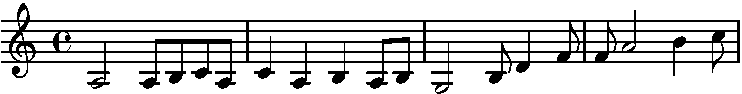
\includegraphics[width=0.95\textwidth]{examples/iter1/melody.cropped.pdf}
    \end{center}
    \caption[Example melody from the first iteration generator, following the no-large-jumps rule but without meaningful structure.]{Example melody of the first iteration melody generator. This follows the simple rule of no large jumps, but follows no meaningful structure or phrasing. \examplelink.}\label{fig:iter1_melody}
  \end{example}

  In Example~\ref{fig:iter1_register} you can see what happens when the generated melody is longer. It will tend to go beyond what an instrument will be able to play. You can see this clearly in \textit{bar 6 through 16} (the entire 2nd and 3rd system\footnote{a system is a line of music, analogous to a line in a paragraph}), where there are very long ledger lines. Some of these notes are not even available on the grand piano.

  \begin{example}
    \begin{center}
      
\includegraphics[width=0.95\textwidth]{examples/iter1/register.cropped.pdf}
    \end{center}
    \caption[Melody showing how the octave is not restricted and the melody wanders outside a playable range.]{Melody showing how the octave is not restricted and the melody wanders outside a playable range. \examplelink.}\label{fig:iter1_register}
  \end{example}

  Another useful feature that was included was the ability to generate more voices at the same time. This feature was quite primitive since the voices were generated independently and did not adhere to any harmony, however it can be a good skeleton to use later if we get to the point that we want to actually harmonize with the melody we generate. In Example~\ref{fig:iter1_voices} you can see how four voices are generated with their own rhythmic restrictions. The bottom voice only has whole notes, the second lowest one has only half-notes, the second highest has only quarter notes, and the top voice has a combination of several note types.


  \begin{example}
    \begin{center}
      
\includegraphics[width=0.70\textwidth]{examples/iter1/voices.cropped.pdf}
    \end{center}
    \caption[Generated multiple voices with different rhythmic restrictions, but without coherent harmony.]{Melody showing how we can generate multiple voices with different rhythmic restrictions. However there is no coherent harmony here every note is placed without regard of the other notes. \examplelink.}\label{fig:iter1_voices}
  \end{example}

\section{Discussion}
  As we can see the first iteration shows a promising proof of concept, however it is quite limited and needs lots of improvement before we have a good system for melody generation.

  The main problem is not only that the output is weak, but also that the internal representation is too poor to improve the output in a systematic way. The generator can place notes in a key and keep the intervals relatively small, but it has no explicit way to describe motifs, phrase structure, cadence, rests, or harmonic relationships between voices. This makes the output feel random, and it also makes the code hard to extend cleanly.

\section{Specifications for next iteration}
  Based on the issues observed in the first iteration, the next step should not only be to generate more notes, but to improve the internal modelling such that the melody can begin to have some actual structure. The second iteration therefore needs to improve both the software representation and the musical behaviour of the generator.

  \begin{itemize}
    \item Introduce more explicit musical objects such as motifs, bars, and phrases, so that the code can represent grouped musical material instead of only a flat stream of notes.
    \item Add some self-similarity by generating and reusing a motif, so the melody starts to feel more coherent from bar to bar.
    \item Make the phrase ending more resolved, preferably by steering the melody toward a more convincing tonic ending.
    \item Improve the handling of notes, durations, keys, and scales so that the code becomes easier to read, reason about, and extend.
  \end{itemize}
